\chapter{Applicazione}
\label{chapter:app}
L'applicazione sviluppata svolge principalmente la funzione di raccoglimento di qualsiasi dato utile alla classificazione.
È possibile racchiudere le funzionalità offerte in
\begin{itemize}
    \item raccoglimento di dati per l'analisi dell'attività.
    \item raccoglimento di dati per l'apprendimento.
    \item raccoglimento di dati aggiuntivi.
\end{itemize}
L'applicazione offre la compatibilità con il sistema operativo \textit{Android}, in particolar modo con tutte le versioni di Android che supportano la 
versione delle API 16 o superiore (ovvero Android 4.1, del 2012, o versioni successive). 
Nella pratica, al momento della stesura di questa relazione, ciò assicura il funzionamento dell'app sul 99,8\% dei dispositivi Android.
\begin{figure}[H]
    \centering
    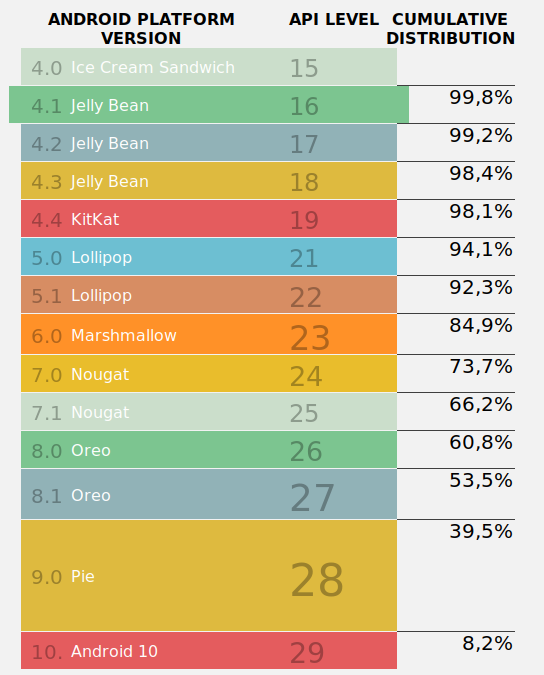
\includegraphics[scale = 0.45]{assets/images/android/compatibility.png}
    \caption{Distribuzione cumulativa delle versioni di Android}
    \label{fig:android-compatibility}
\end{figure}
I linguaggi utilizzati per lo sviluppo sono stati \textit{Java} per quanto riguarda l'aspetto programmativo, mentre \textit{XML} per tutti i
layout.



\section{Interfaccia}
Si è voluta dare un'interfaccia minimale sviluppata secondo le linee guida dell'ormai conosciuto Material Design \cite{material}, un 
linguaggio visivo che sintetizza i principi classici del buon design ispirandosi al mondo fisico.

Le 3 sezioni presenti suddividono con esattezza le 3 funzionalità offerte: 
l'analisi dell'attività, l'apprendimento di una attività e l'inserimento di informazioni aggiuntive.
\begin{figure}[H]
    \centering
    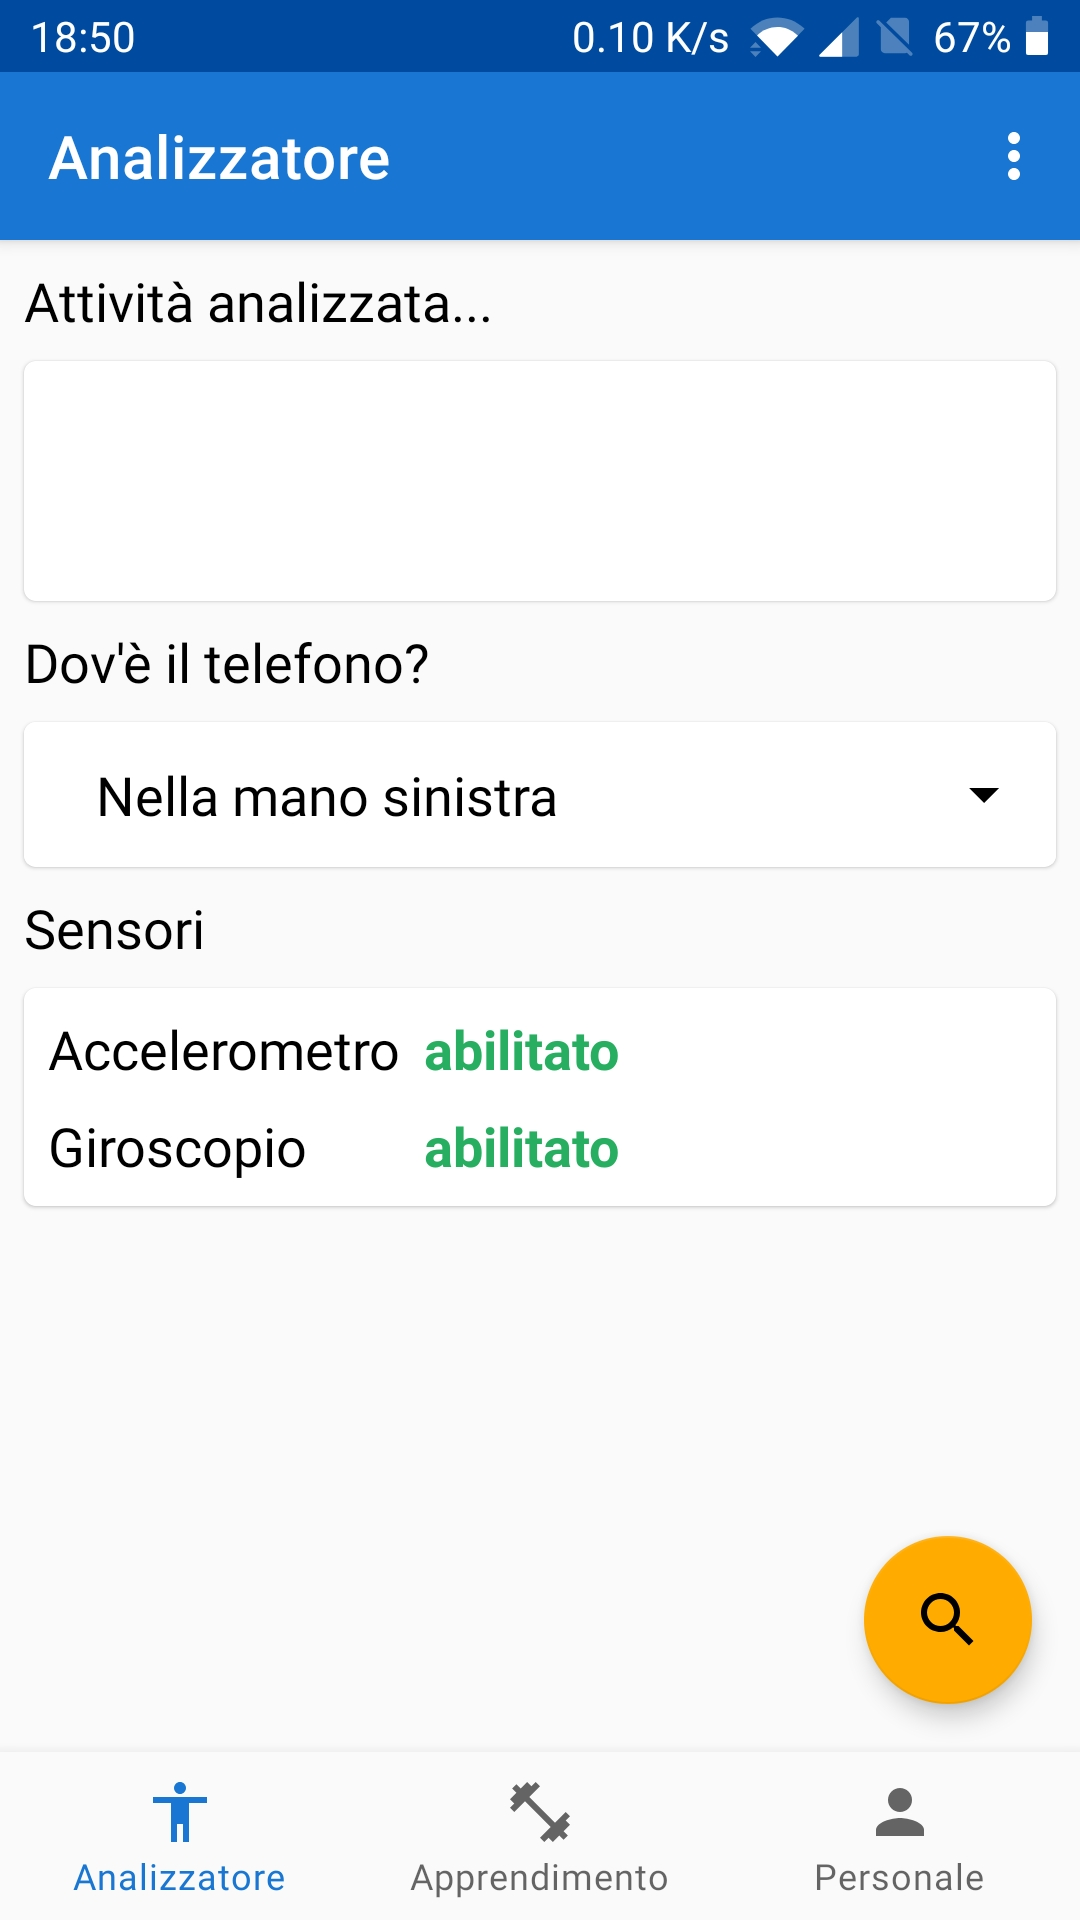
\includegraphics[scale = 0.10]{assets/images/screenshots/1a_Init.jpg}
    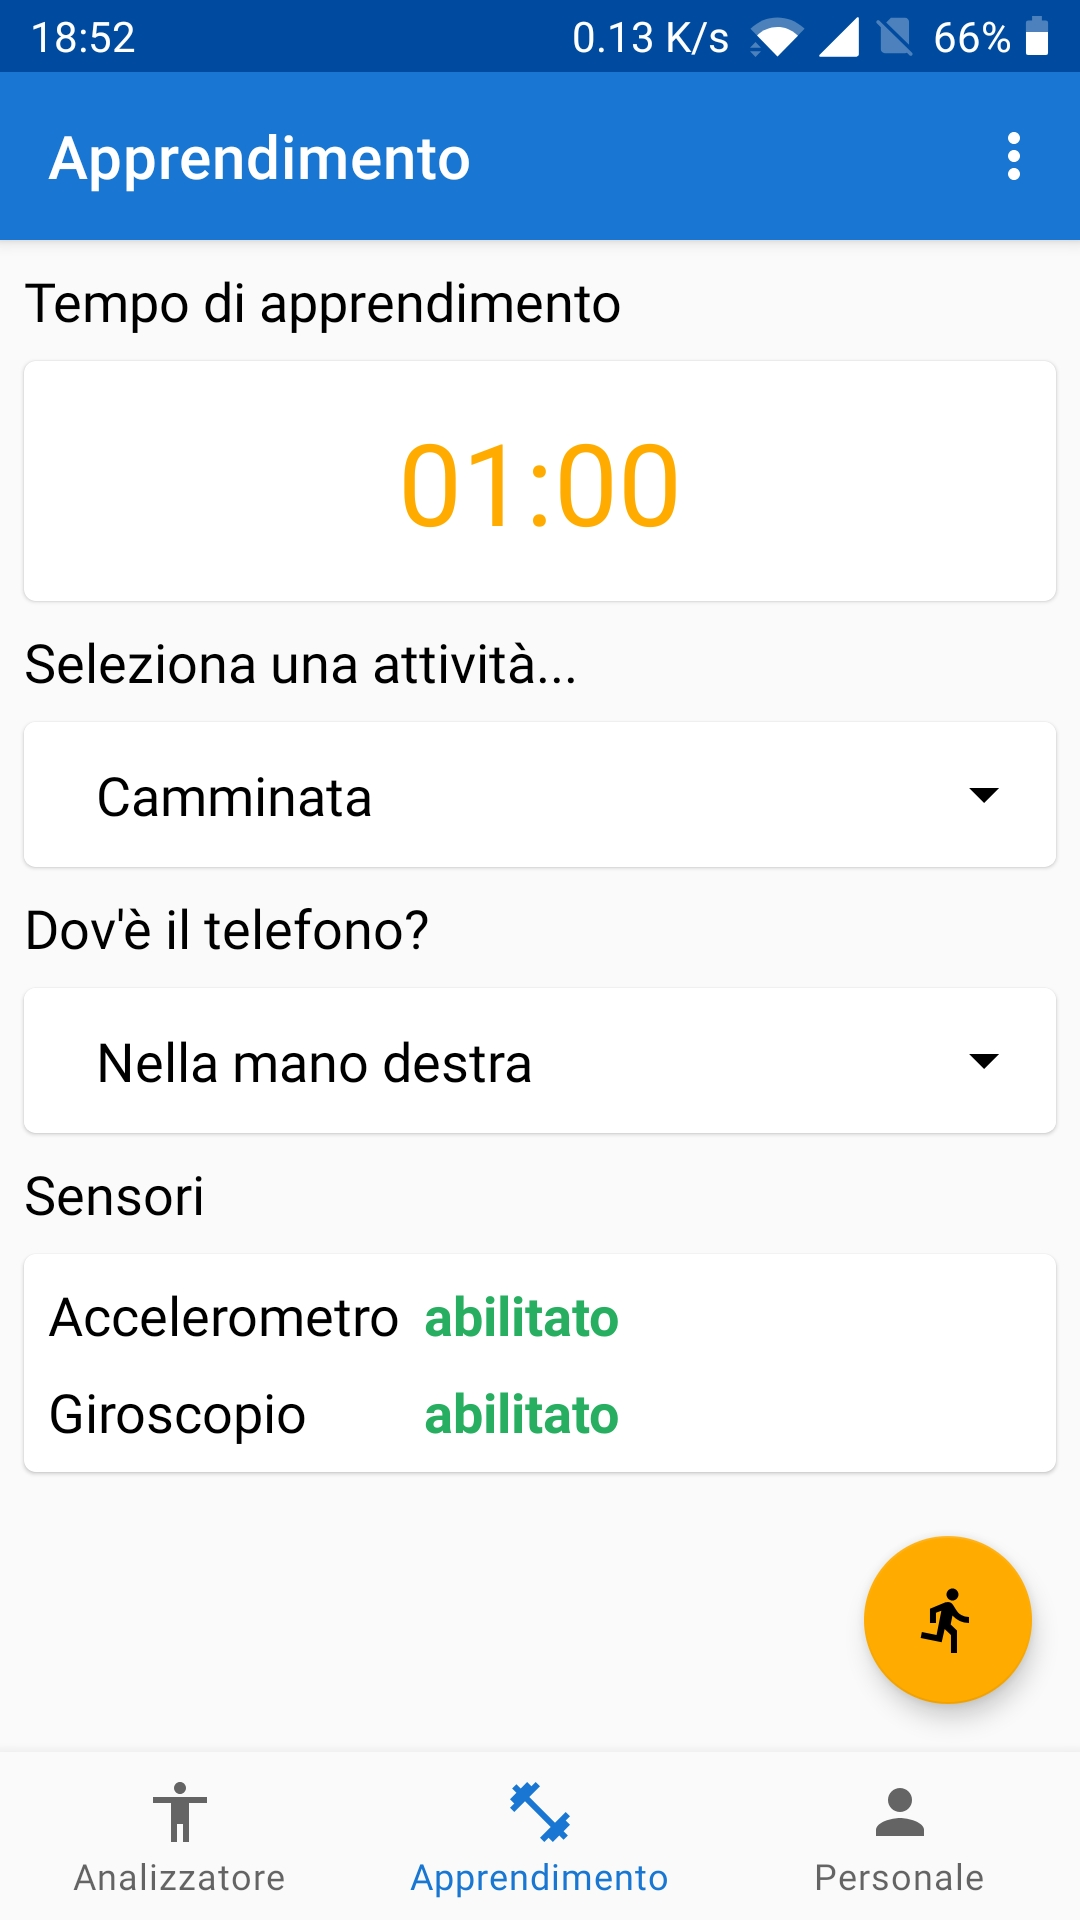
\includegraphics[scale = 0.10]{assets/images/screenshots/2a_Init.jpg}
    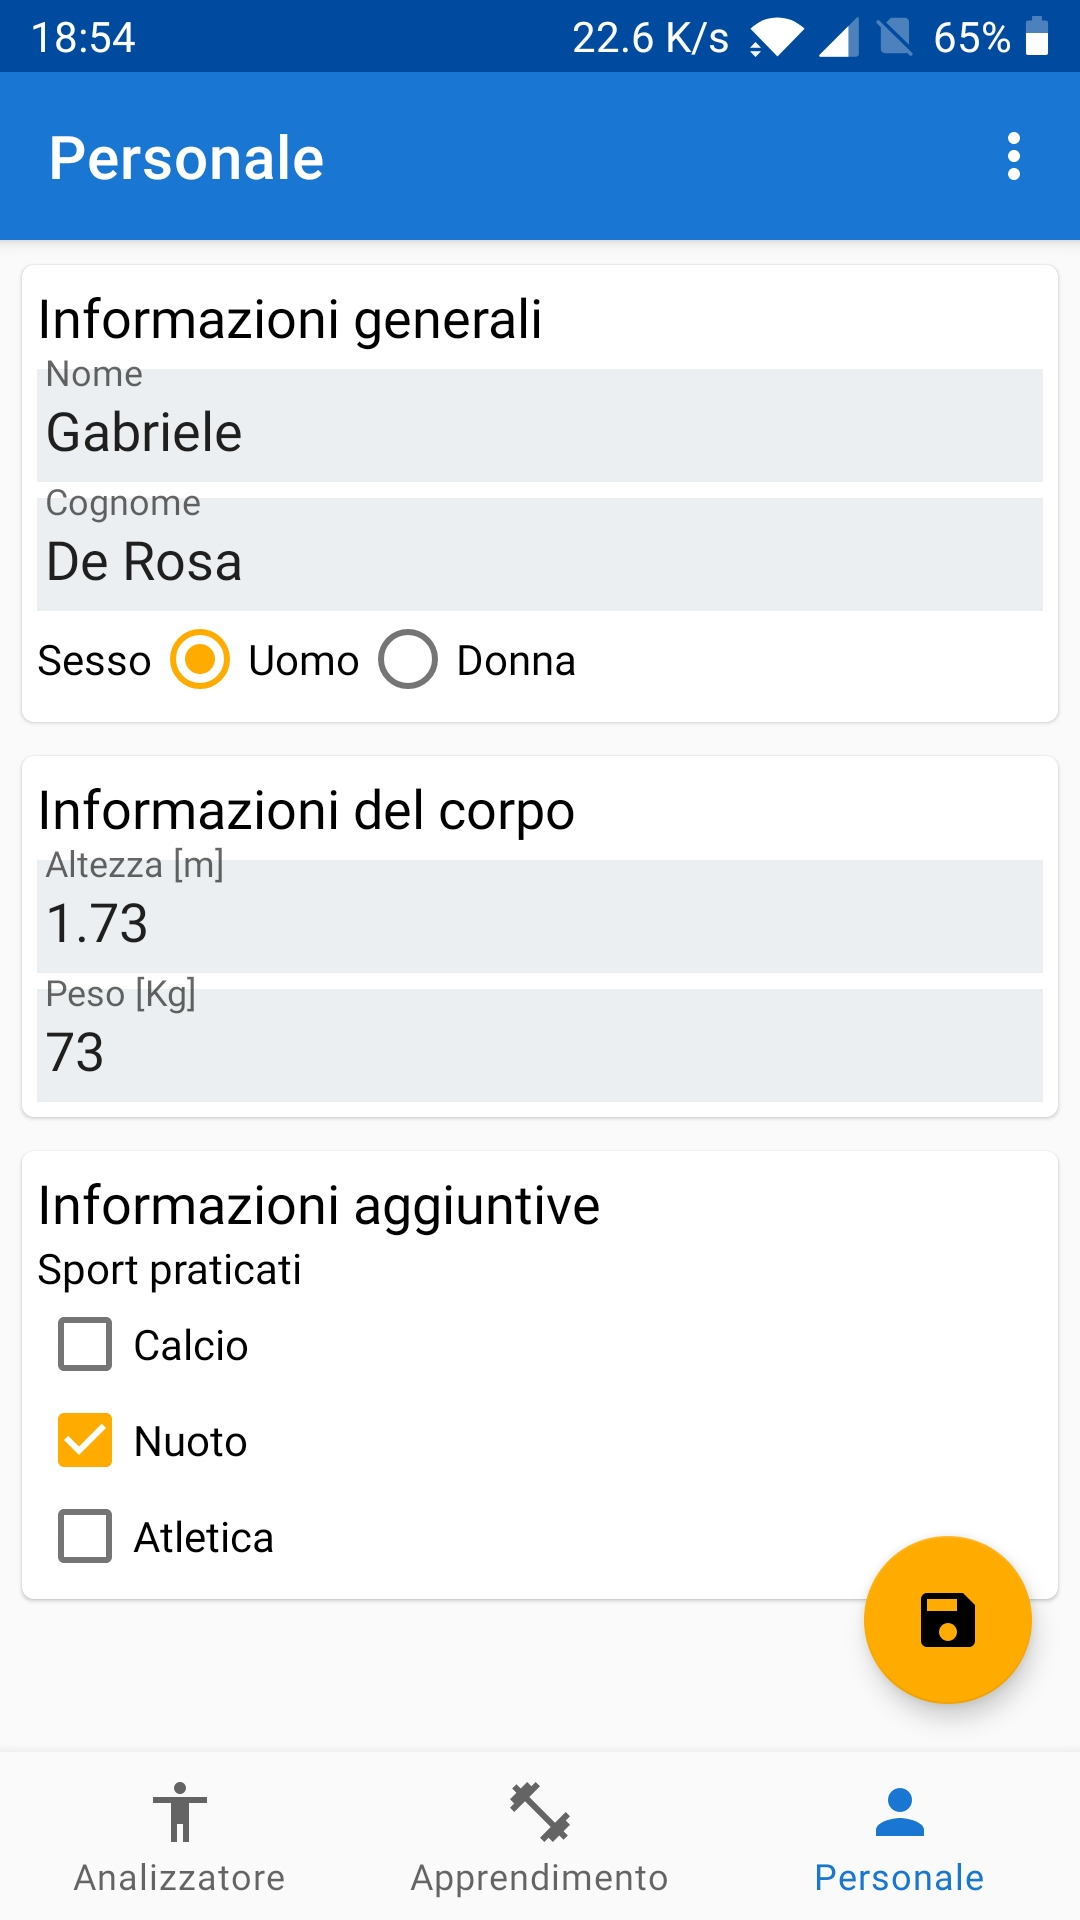
\includegraphics[scale = 0.10]{assets/images/screenshots/3a_Init.jpg}
    \caption{Le 3 sezioni principali dell'applicazione}
    \label{fig:screenshots}
\end{figure}

\subsection{Sezione di analisi}
Nella sezione di analisi è possibile avviare un processo che sarà in grado di ipotizzare l'attività che si sta svolgendo.
L'insieme delle azioni svolte in questa sezione sono divisibili in 4 fasi.

\subsubsection{Fase 1: Inizializzazione}
In questa prima fase l'applicazione scarica tramite l'utilizzo delle API (vedi sezione \ref{section:api}) le informazioni relative
alle posizioni del dispositivo che sono disponibili e selezionabili.
L'utente ha la possibilità di selezionare la posizione dove tenere il telefono durante l'attività ed avviare l'analisi.

\subsubsection{Fase 2: Preparazione}
In seguito all'avvio dell'analisi sarà avviato un servizio in foreground \cite{services} dell'applicazione che si occuperà di svolgere tutte le azioni 
necessarie per le fasi seguenti. La UI continuerà ad essere aggiornata con le informazioni ricevute dal servizio.

Il service appena avviato si occuperà di cercare un contatto con il server per stabilire una connessione TCP.

Qualora la connessione avvenisse con successo sarà avviato un conto alla rovescia pensato appositamente in modo da consentire all'utente 
di prepararsi posizionando il dispositivo nella posizione selezionata precedentemente.

\subsubsection{Fase 3: Analisi}
Allo scadere del countdown riservato alla preparazione è avviata l'analisi vera e propria ed inizia anche lo scambio dati con il server.

I sensori abilitati iniziano la raccolta dei dati ed ogni informazione ottenuta viene inviata.

\subsubsection{Fase 4: Predizione}
Durante l'analisi il server risponde con diversi messaggi. Tra i principali troviamo il messaggio di conferma di ricezione di un dato, 
ma soprattutto è rilevante il messaggio contenente l'attività che è stata ipotizzata.

\begin{figure}[H]
    \centering
    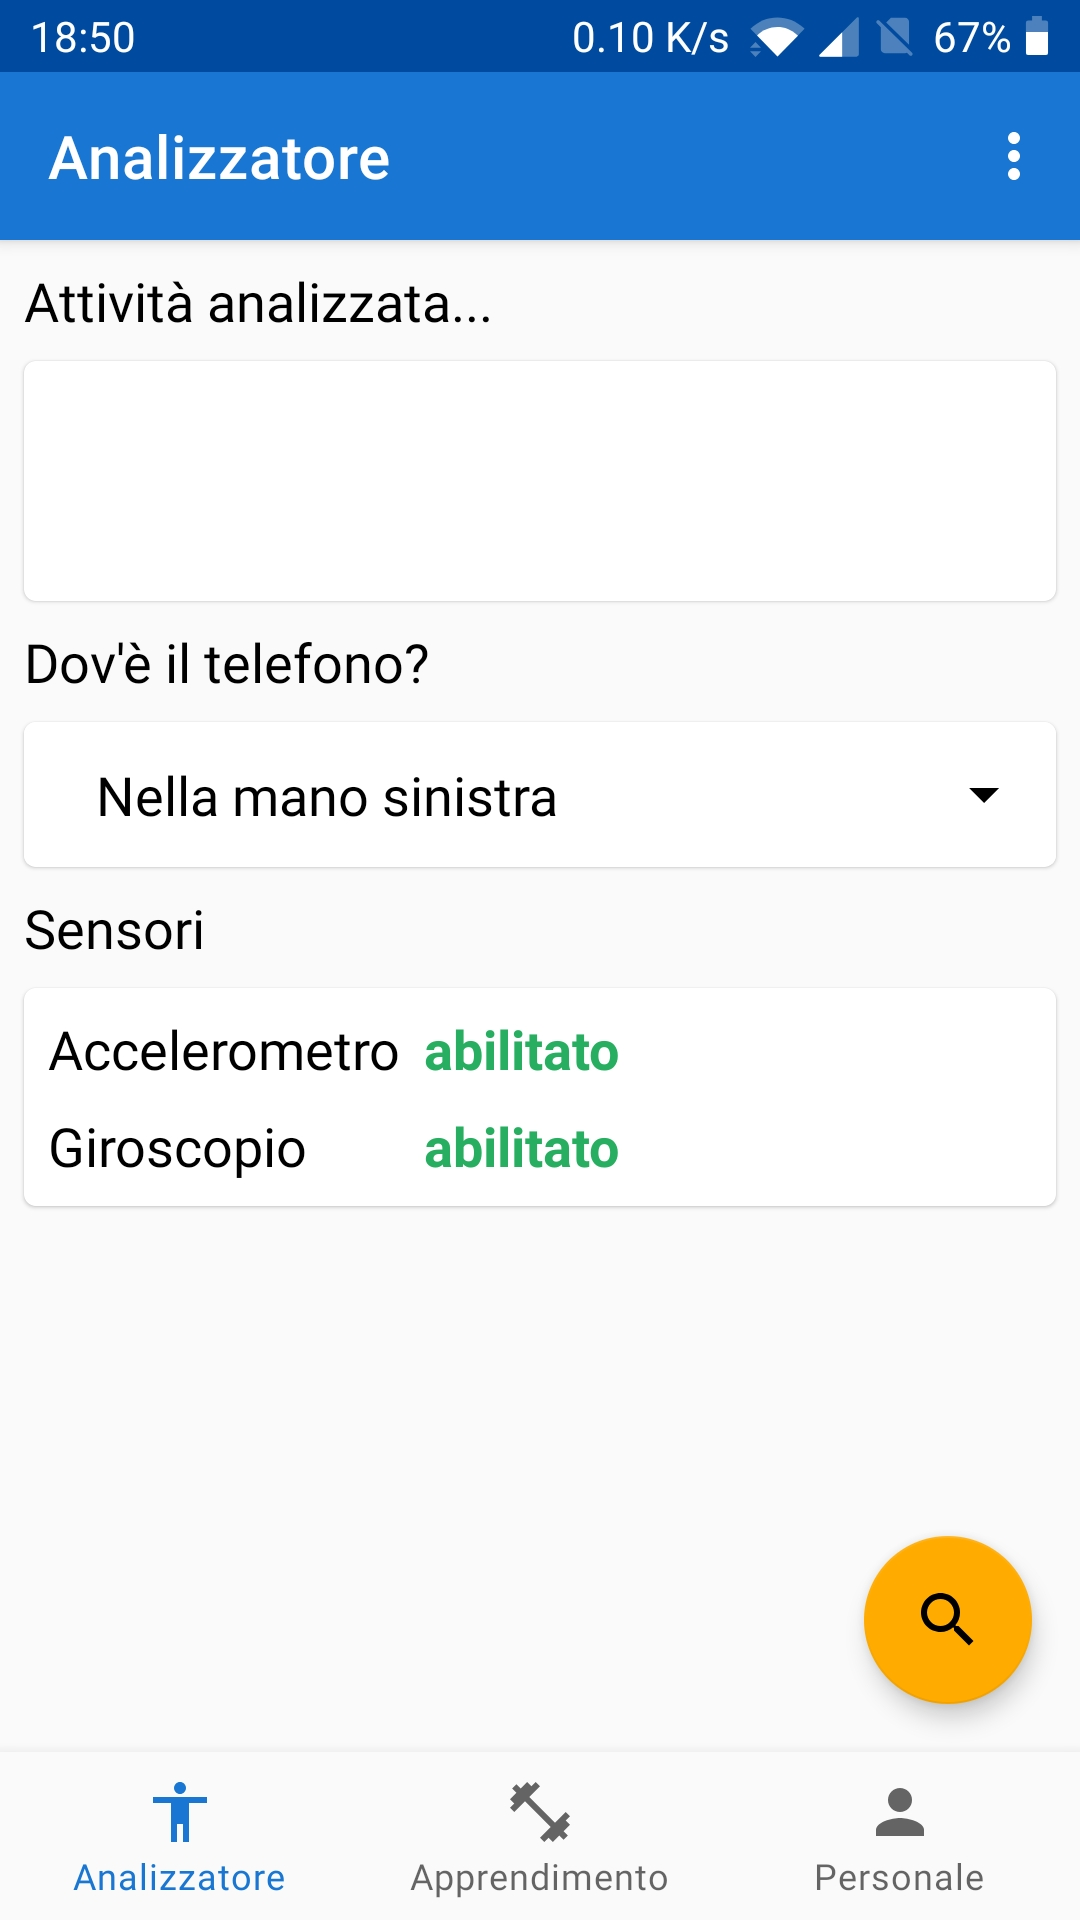
\includegraphics[scale = 0.10]{assets/images/screenshots/1a_Init.jpg}
    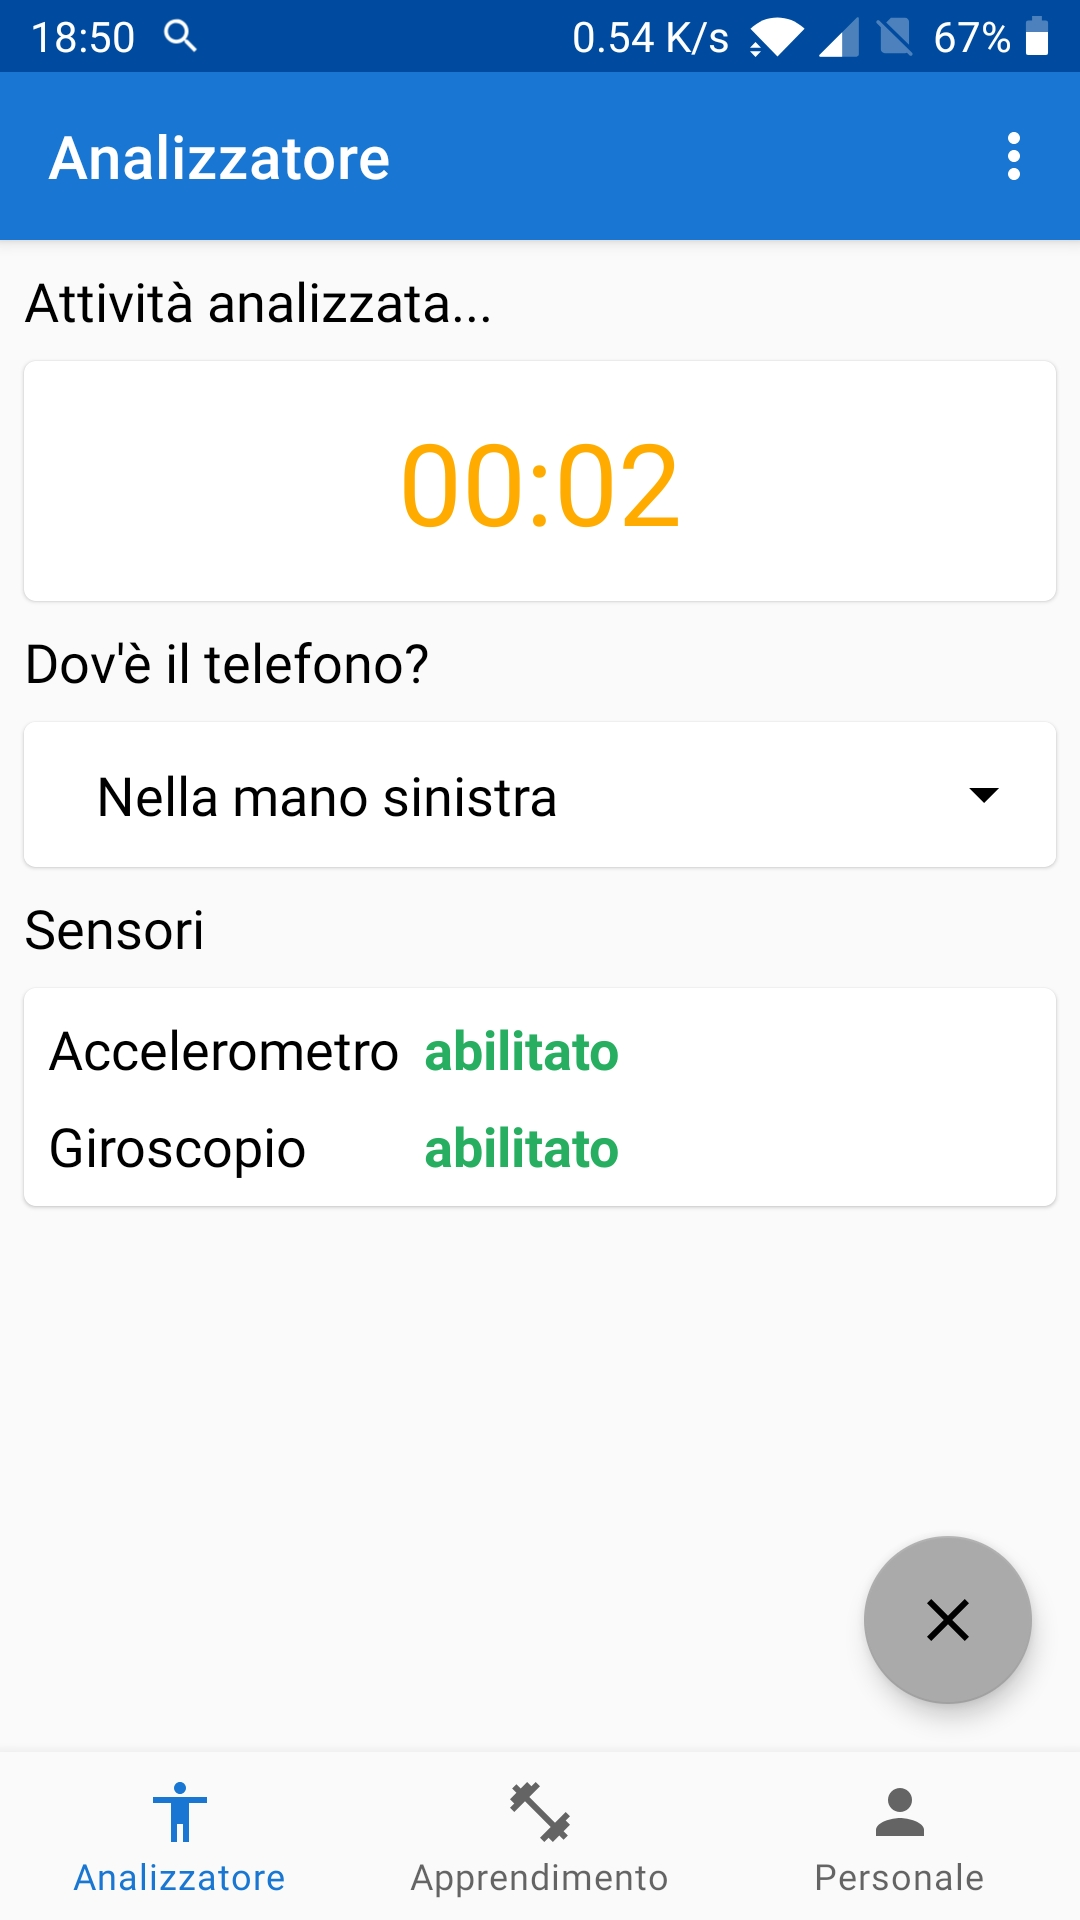
\includegraphics[scale = 0.10]{assets/images/screenshots/1b_Preparation.jpg}
    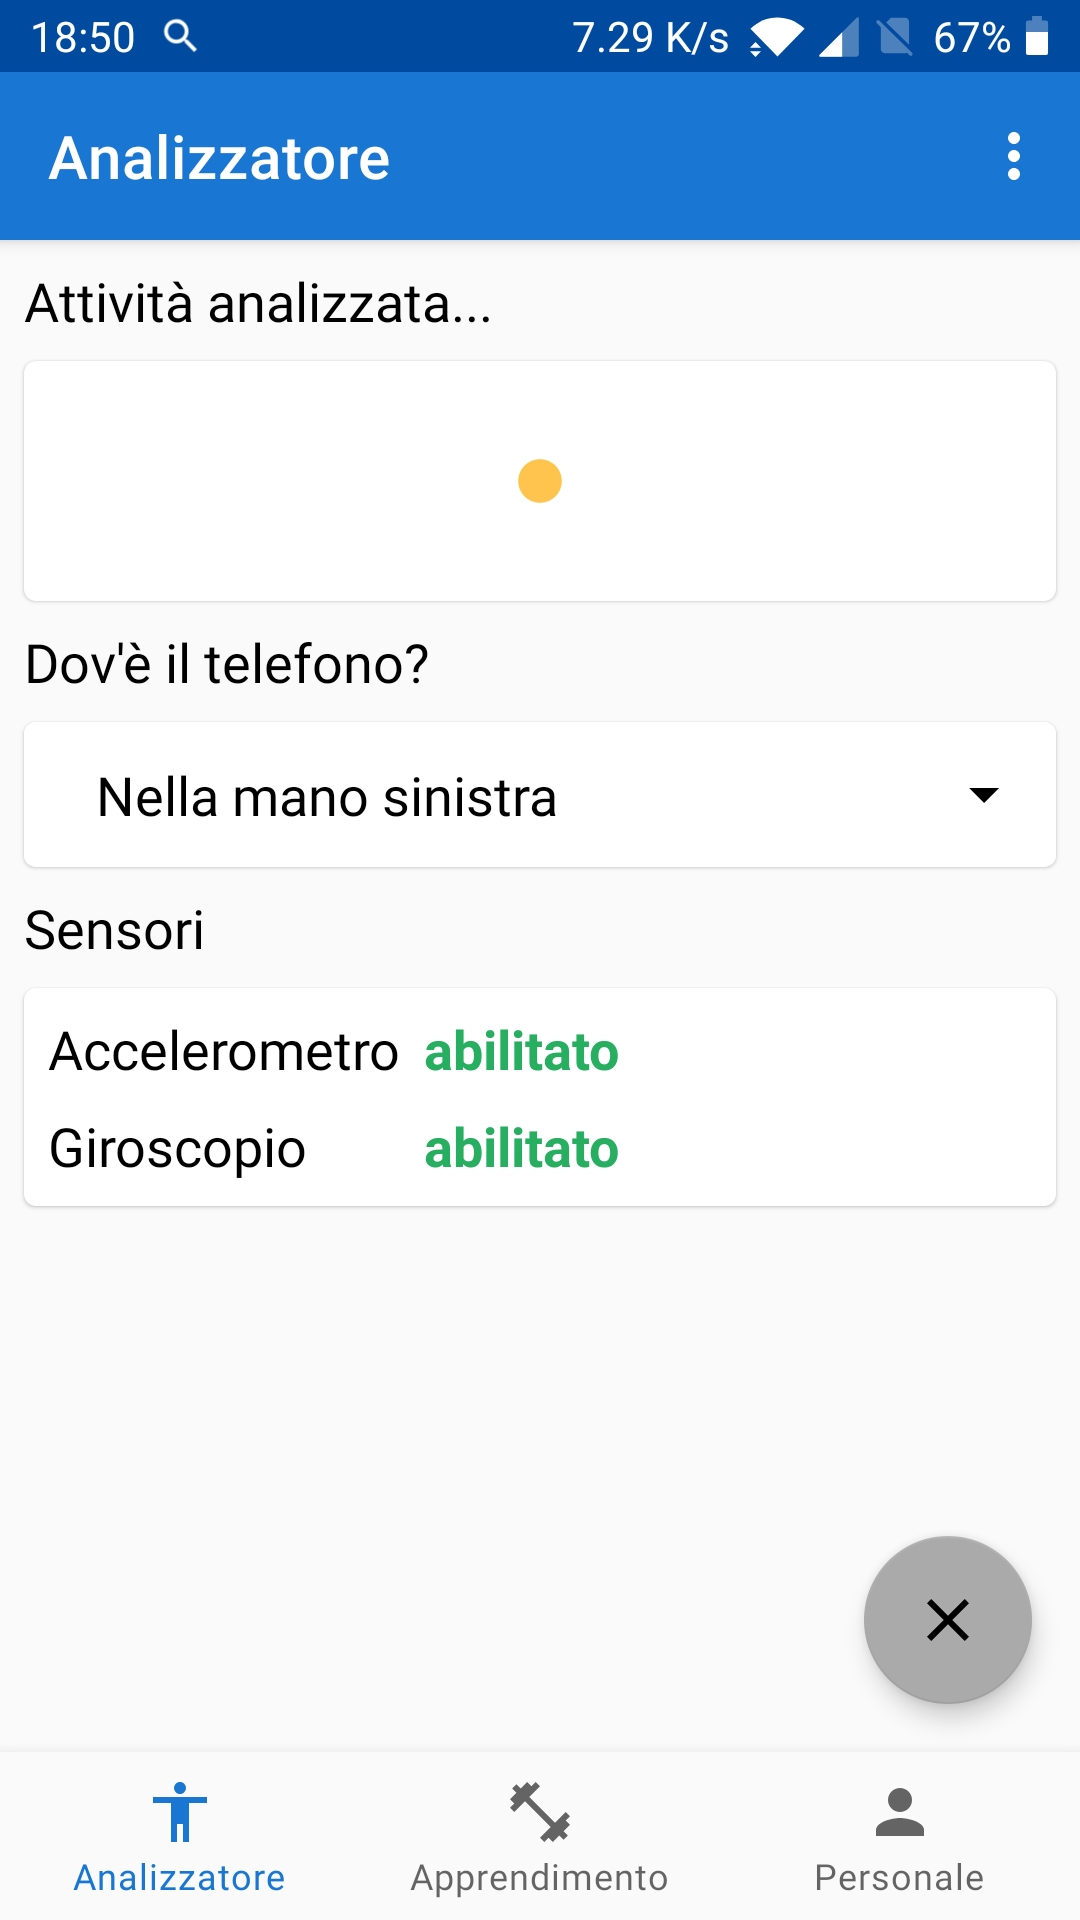
\includegraphics[scale = 0.10]{assets/images/screenshots/1c_Analysis.jpg}
    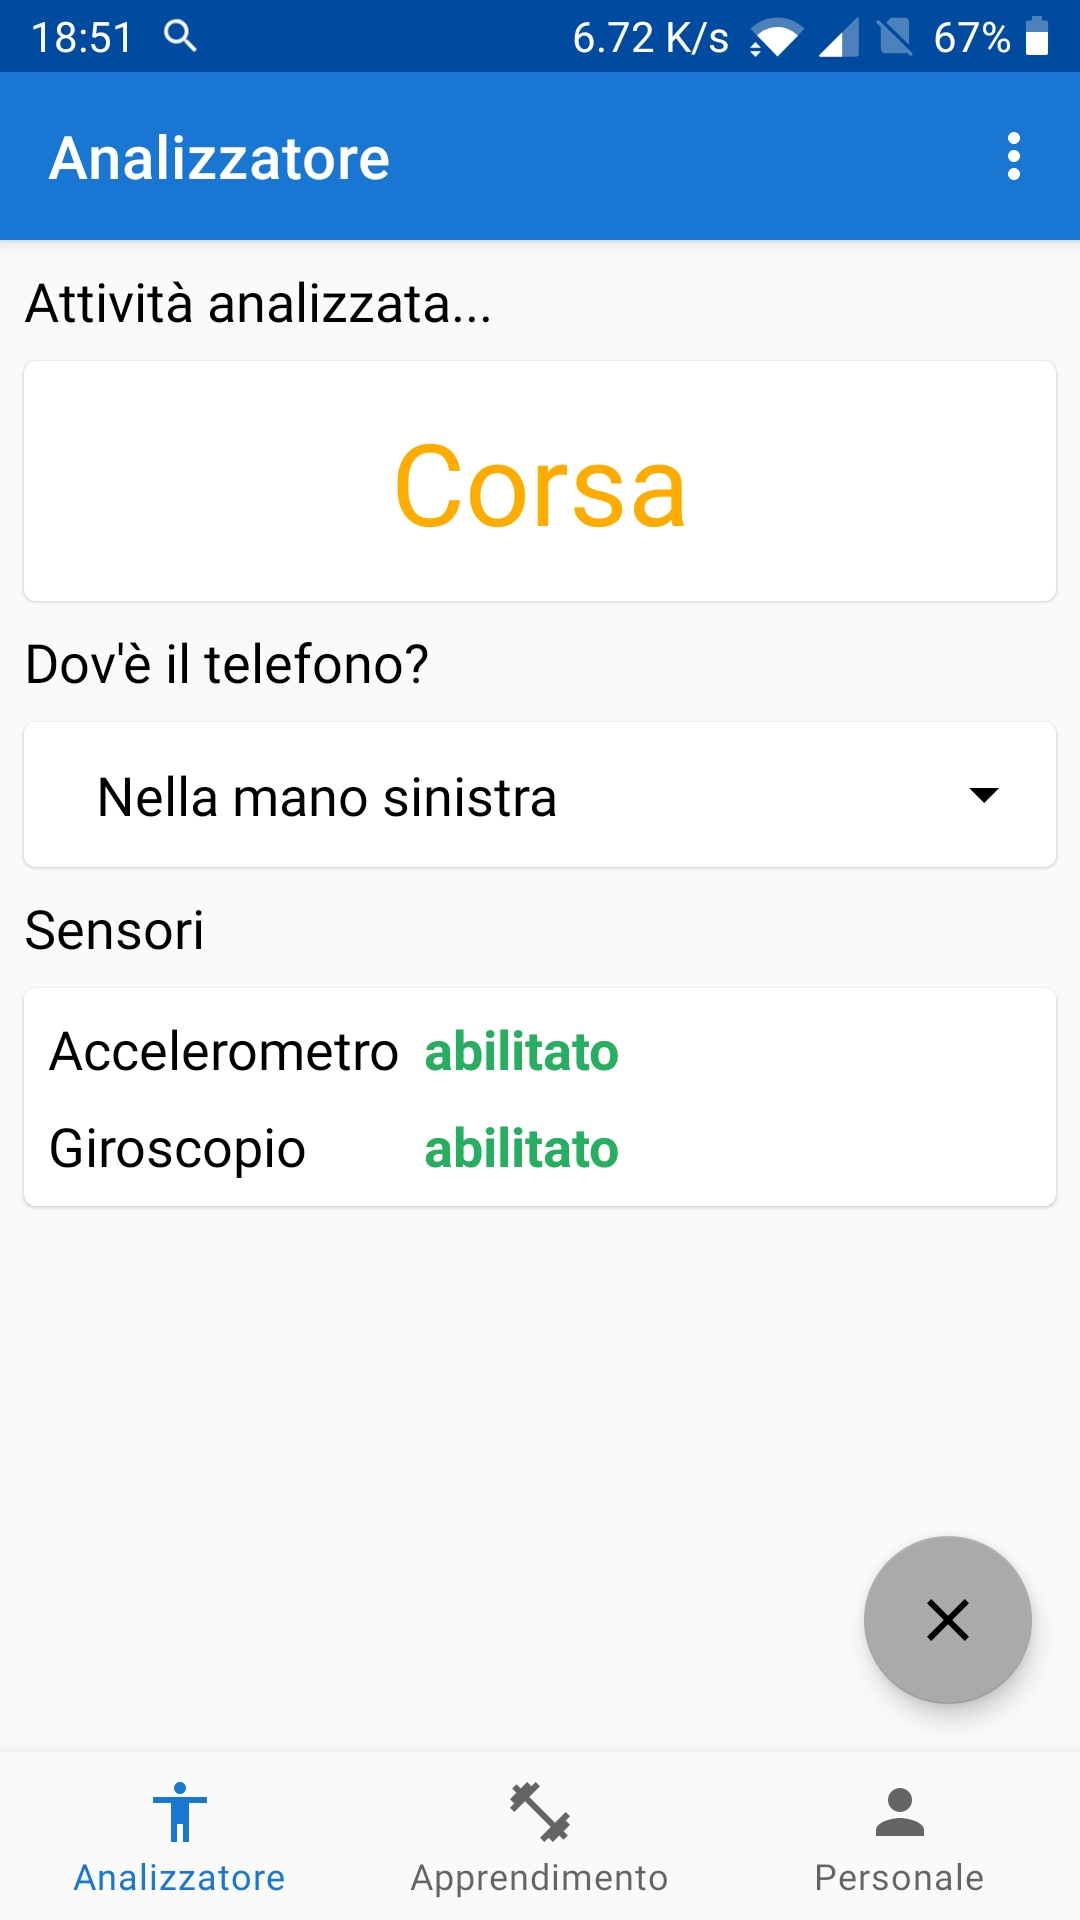
\includegraphics[scale = 0.10]{assets/images/screenshots/1d_Prediction.jpg}
    \caption{Le 4 fasi dell'analisi}
    \label{fig:screenshots_analysis}
\end{figure}


\subsection{Sezione di apprendimento}
Nella sezione di apprendimento è possibile avviare un processo in grado di raccogliere dei dati sensoriali associandoli ad una
determinata attività. 

L'obiettivo sarà poi utilizzare questi dati per effettuare il \textit{train} della dati per la creazione di un modello. In questa fase si da 
piena fiducia all'utente sulla correttezza dei dati inseriti.

L'insieme delle azioni svolte in questa sezione sono divisibili in 3 fasi.

\subsubsection{Fase 1: Inizializzazione}
In questa prima fase l'applicazione scarica tramite l'utilizzo delle API (vedi sezione \ref{section:api}) diverse informazioni:
\begin{itemize}
    \item le informazioni relative alle posizioni del dispositivo selezionabili
    \item la lista di attività addestrabili e il tempo necessario per il loro apprendimento
\end{itemize}

L'utente dovrà quindi selezionare la posizione dove tenere il telefono durante l'attività e l'attività che andrà a svolgere 
prima di avviare l'apprendimento.

\subsubsection{Fase 2: Preparazione}
In seguito all'avvio dell'apprendimento sarà avviato un servizio in foreground \cite{services} dell'applicazione che si occuperà di svolgere 
tutte le azioni necessarie per le fasi seguenti. La UI continuerà ad essere aggiornata con le informazioni ricevute dal servizio.

Il service appena avviato si occuperà di cercare un contatto con il server per stabilire una connessione TCP.

Qualora la connessione avvenisse con successo sarà avviato un conto alla rovescia pensato appositamente in modo da consentire all'utente 
di prepararsi posizionando il dispositivo nella posizione selezionata precedentemente.

\subsubsection{Fase 3: Apprendimento}
Allo scadere del countdown riservato alla preparazione sono avviati in parallelo un nuovo conto alla rovescia 
e tutti i sensori  per la raccolta dei dati.

I dati raccolti dai sensori sono inviati costantemente al server. Una volta scaduto il conto alla rovescia la raccolta dei dati sarà terminata.

\begin{figure}[H]
    \centering
    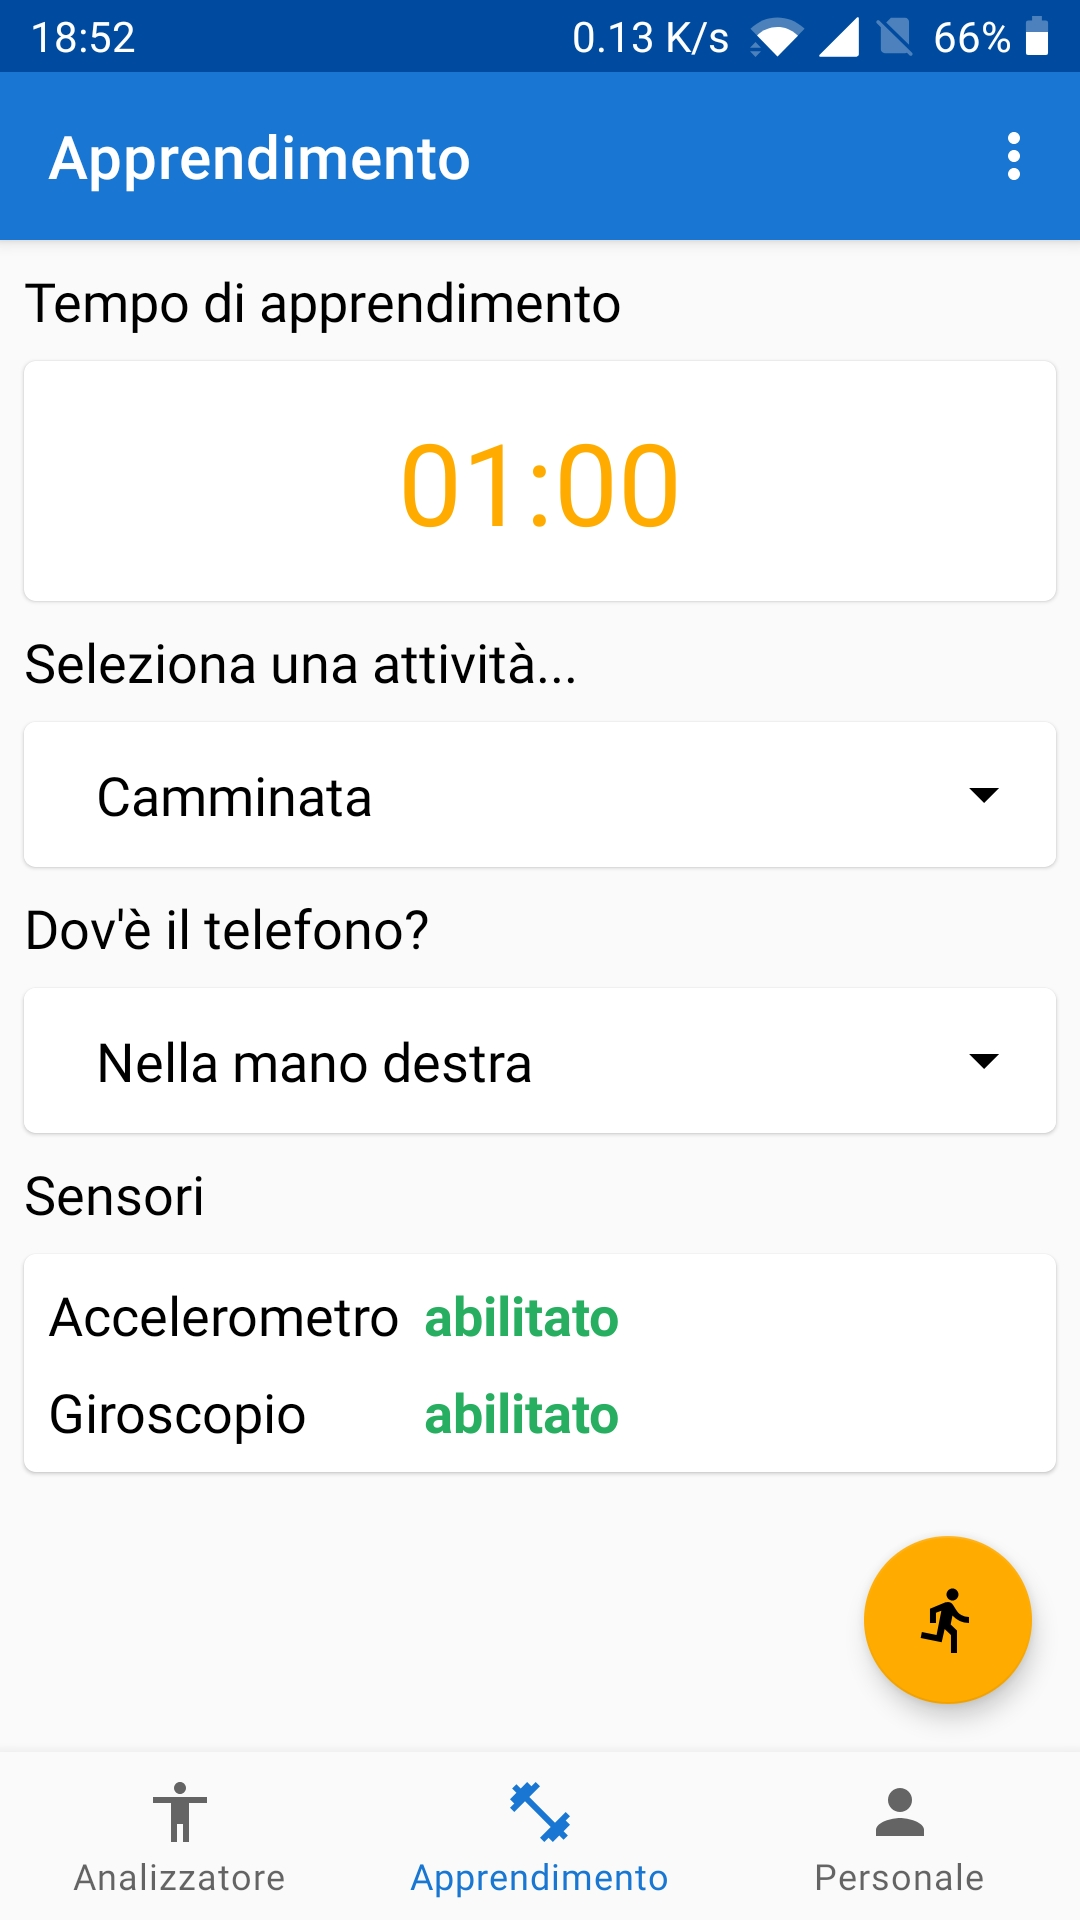
\includegraphics[scale = 0.10]{assets/images/screenshots/2a_Init.jpg}
    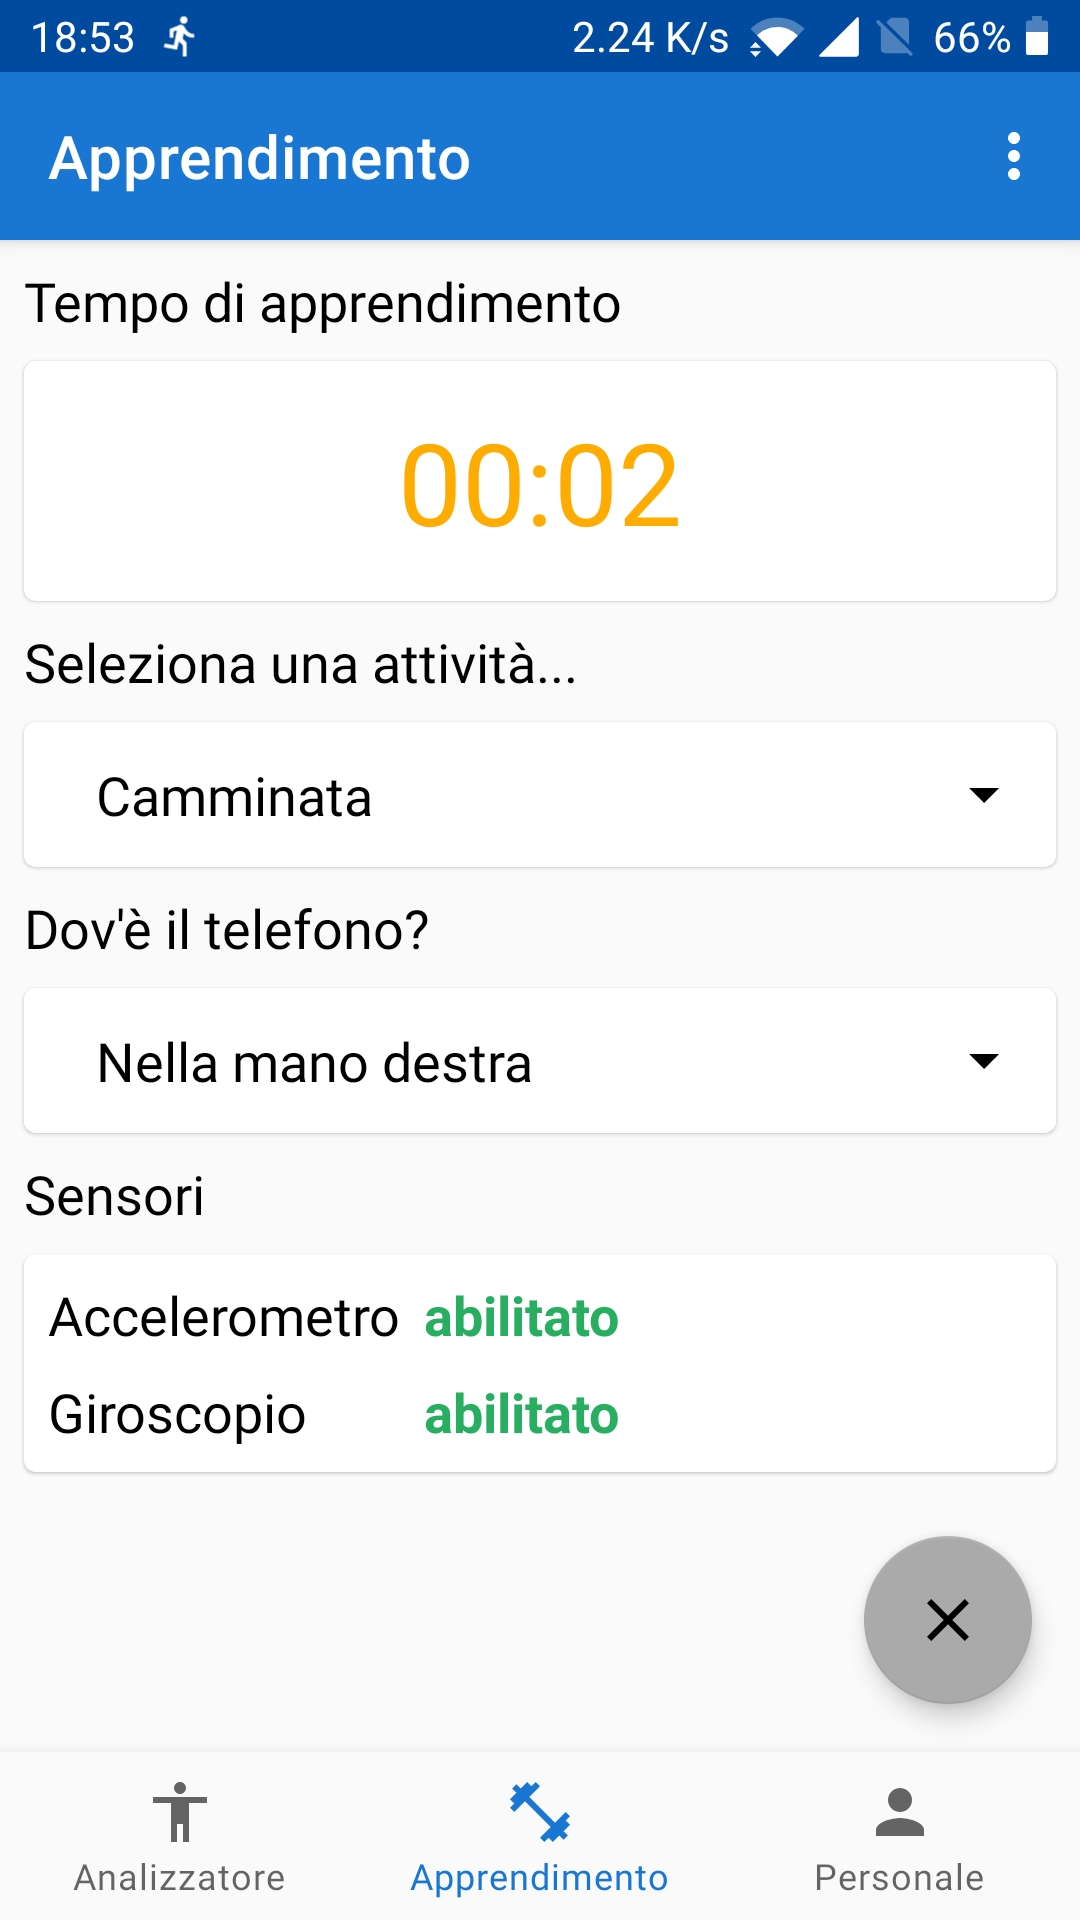
\includegraphics[scale = 0.10]{assets/images/screenshots/2b_Preparation.jpg}
    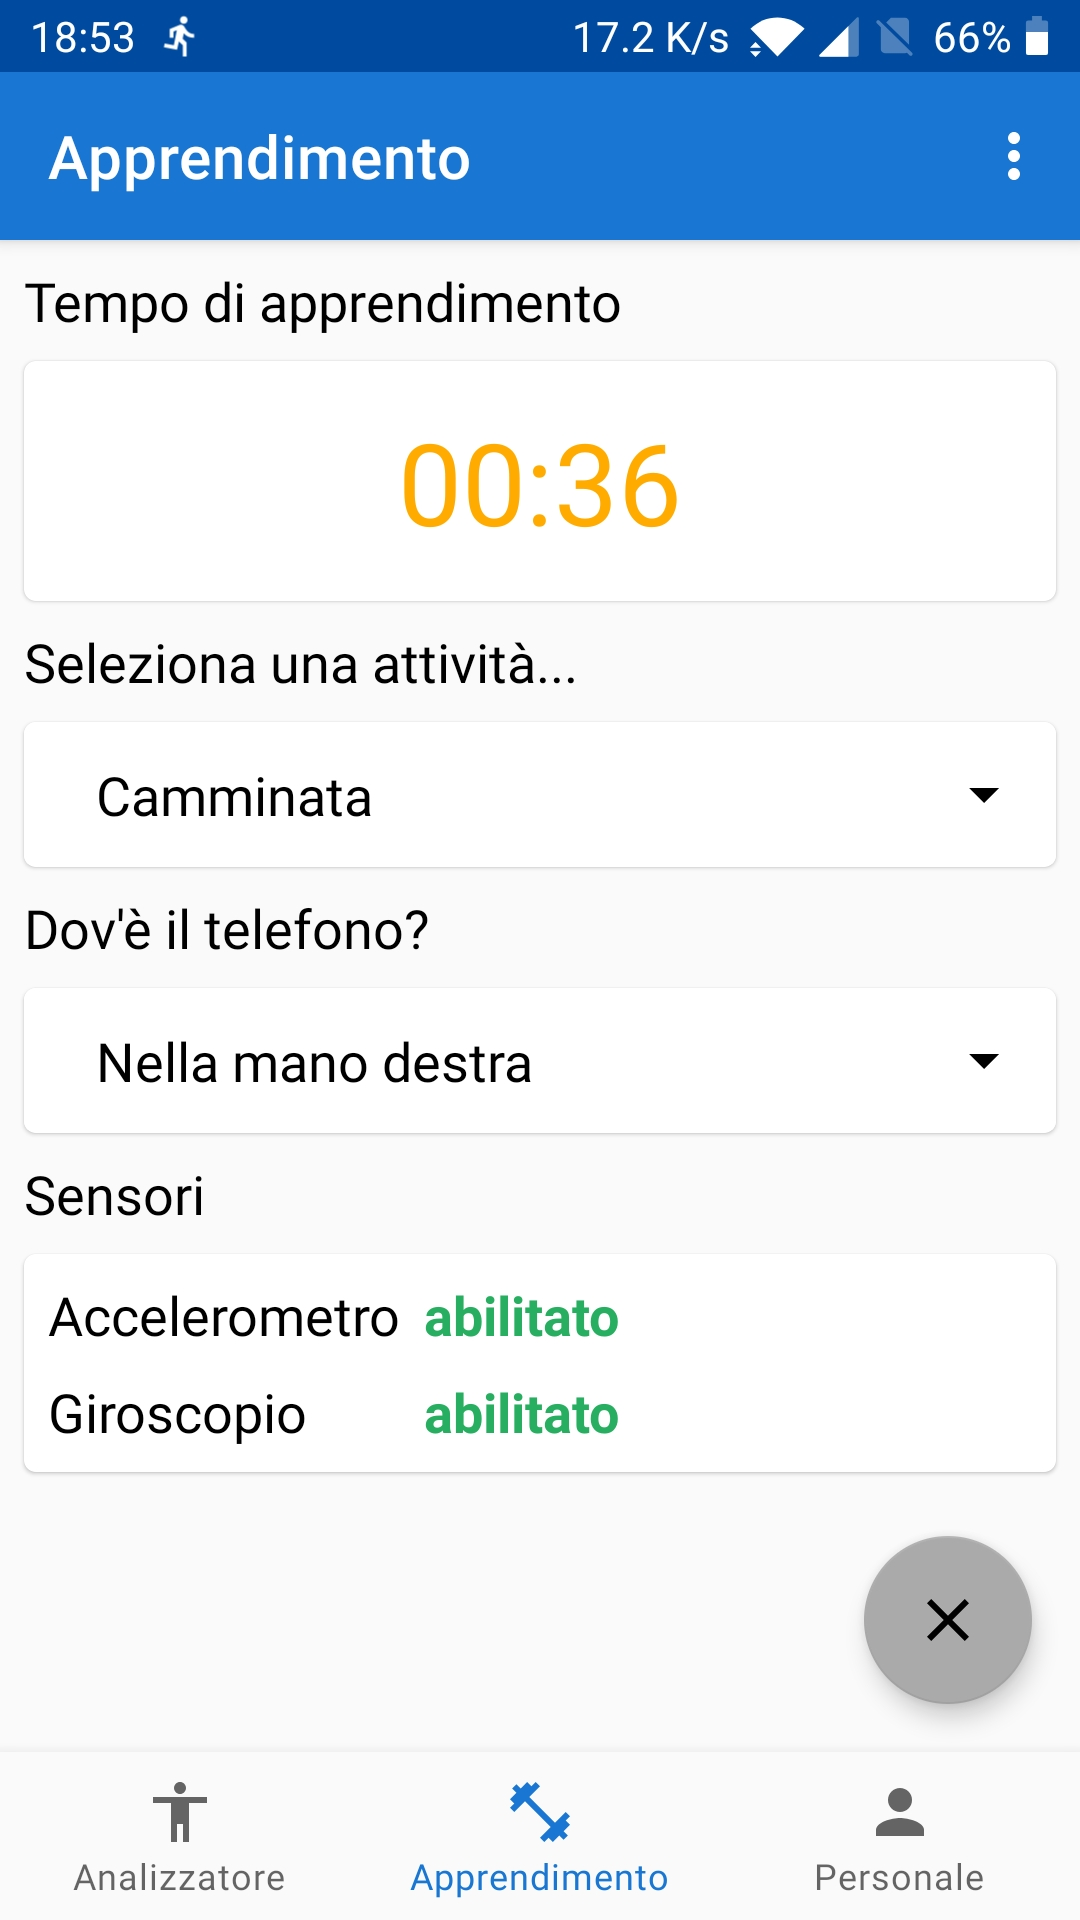
\includegraphics[scale = 0.10]{assets/images/screenshots/2c_Learning.jpg}
    \caption{Le 3 fasi dell'apprendimento}
    \label{fig:screenshots_learning}
\end{figure}


\subsection{Sezione per l'inserimento di dati aggiuntivi}
Nella sezione di apprendimento è presente un modulo di inserimento dati utile per permettere all'utilizzatore di 
inserire dati aggiuntivi relativi alla sua persona. Potenzialmente si potrebbe pensare che questi dati saranno poi utilizzabili
per una classificazione più approfondita.

Un aspetto particolare di questo modulo consiste nella sua dinamicità. Tutte la sua intera struttura è generata programmativamente 
tramite le informazioni ottenute in fase di creazione tramite una chiamata alle API (vedi sezione delle \ref{section:api}).

\begin{figure}[H]
    \centering
    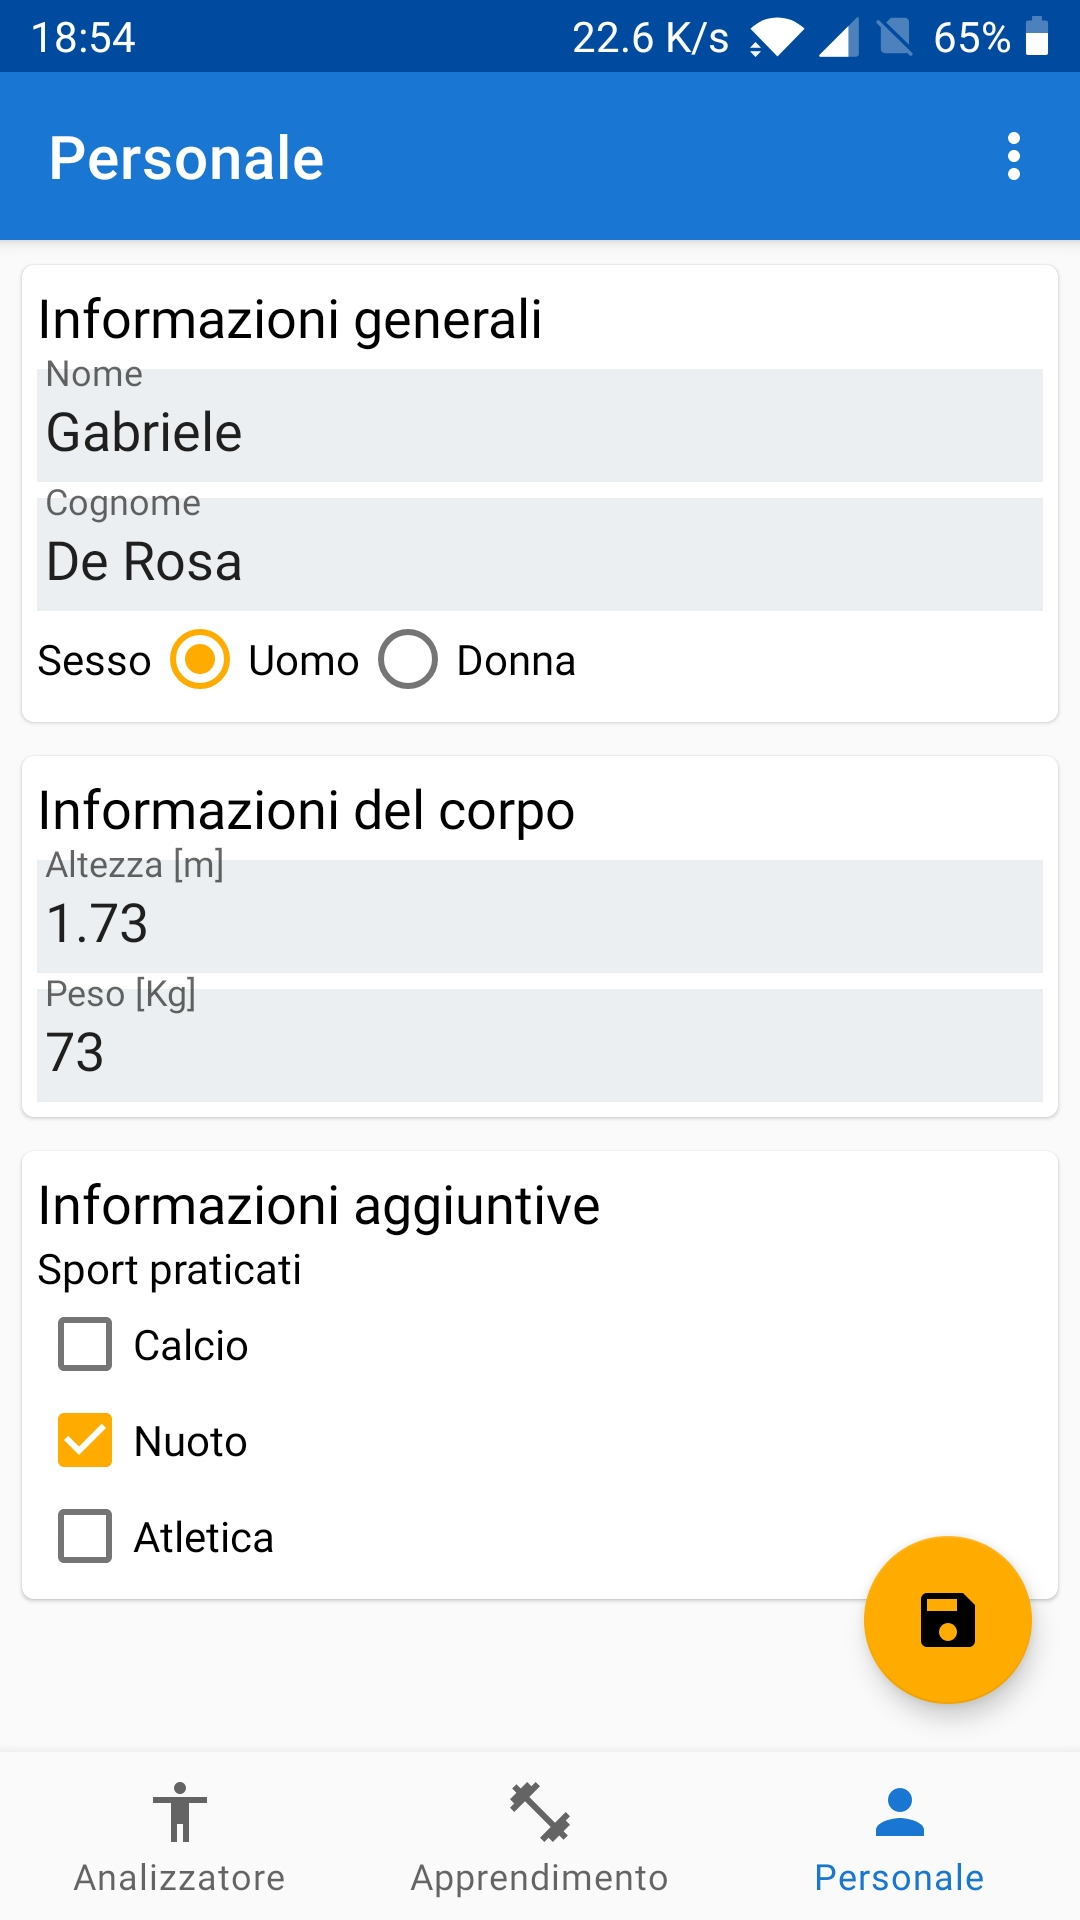
\includegraphics[scale = 0.10]{assets/images/screenshots/3a_Init.jpg}    
    \caption{Il modulo di inserimento dati generato programmativamente}
    \label{fig:screenshots_personal}
\end{figure}


\subsection{Feedback sonoro}
Oltre a quanto si vede sull'interfaccia dell'applicazione, essa fornisce un feedback sonoro mediante il sintetizzatore vocale
del dispositivo che fornisce tutte le informazioni visualizzate sulla UI. Questa necessità dipende dal fatto che l'utilizzo potrebbe avvenire 
dopo aver posizionato il dispositivo in modo da impedirne la visualizzazione delle informazioni (ad esempio in tasca).



\section{Implementazione}
Gli aspetti programmativi che più interessano sono indubbiamente quelli legati all'accesso alle API, alla gestione dei conti 
alla rovescia, alle comunicazioni con il server, al feedback sonoro e alla raccolta dei dati con i principali sensori di movimento.

\subsection{Accesso alle API}
Le chiamate alle API sono fatte utilizzando la librerie Retrofit \cite{retrofit}.


\subsection{Countdown Timers}
Per l'implementazione dei conti alla rovescia ho implementato la classe \textit{CountDownTimer} \cite{countdown}
offerta direttamente da Android.


\subsection{Connessione con il server}
Per la connessione al server è stata implementata con l'utilizzo della classe \textit{Socket} \cite{socket}.


\subsection{Feedback sonoro}
La sintetizzazione vocale è stata implementata con le librerie di \textit{text to speech} \cite{tts} offerte da Android.


\subsection{Sensori di movimento}
I sensori di movimento implementati sono accelerometro e giroscopio.


%\section{Scambio dati con il server}